% !TeX root = ../main.tex
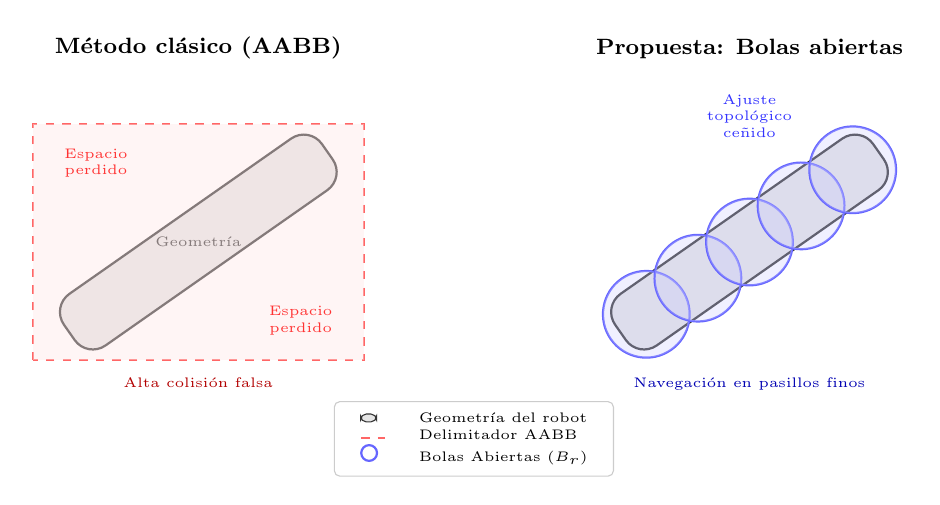
\begin{tikzpicture}[>=stealth, scale=1.0, every node/.style={font=\small}]

% Estilo para el eslabón del robot (geometría original)
\tikzset{
    robotlink/.style={
        draw=black!80, 
        fill=gray!20, 
        rounded corners=8pt, 
        thick
    }
}

% =============================================
% PANEL IZQUIERDO: Bounding Box Clásica (AABB)
% =============================================
\begin{scope}[shift={(-3.5,0)}]
    \node[anchor=south, font=\bfseries\footnotesize] at (0, 2.2) {Método clásico (AABB)};
    
    % Dibujamos el eslabón inclinado
    \begin{scope}[rotate=35]
        \draw[robotlink] (-2, -0.4) rectangle (2, 0.4);
        \node[font=\tiny, black!80] at (0,0) {Geometría};
    \end{scope}

    % Caja AABB (Rectángulo ortogonal que lo encierra)
    % El brazo rotado 35 grados tiene una caja que lo encierra de aprox 4x3
    \draw[red!60, dashed, thick] (-2.1, -1.5) rectangle (2.1, 1.5);
    \fill[red!10, opacity=0.4] (-2.1, -1.5) rectangle (2.1, 1.5);
    
    % Etiquetas de ineficiencia
    \node[red!80, font=\tiny, text width=1.5cm, align=center] at (-1.3, 1.0) {Espacio perdido};
    \node[red!80, font=\tiny, text width=1.5cm, align=center] at (1.3, -1.0) {Espacio perdido};
    
    \node[anchor=north, font=\tiny, text=red!70!black] at (0, -1.6) {Alta colisión falsa};
\end{scope}

% =============================================
% PANEL DERECHO: Bolas Abiertas (Propuesta)
% =============================================
\begin{scope}[shift={(3.5,0)}]
    \node[anchor=south, font=\bfseries\footnotesize] at (0, 2.2) {Propuesta: Bolas abiertas};
    
    % Dibujamos el eslabón inclinado (mismo ángulo)
    \begin{scope}[rotate=35]
        \draw[robotlink] (-2, -0.4) rectangle (2, 0.4);
    \end{scope}

    % Recubrimiento por bolas (cadena de esferas)
    \begin{scope}[rotate=35]
        \foreach \x in {-1.6, -0.8, 0, 0.8, 1.6} {
            \draw[blue!60, thick] (\x, 0) circle (0.55);
            \fill[blue!20, opacity=0.3] (\x, 0) circle (0.55);
        }
    \end{scope}
    
    % Etiquetas de eficiencia
    \node[blue!80, font=\tiny, text width=1.8cm, align=center] at (0, 1.6) {Ajuste topológico ceñido};
    
    \node[anchor=north, font=\tiny, text=blue!70!black] at (0, -1.6) {Navegación en pasillos finos};
\end{scope}

% =============================================
% LEYENDA CENTRAL
% =============================================
\node[draw=black!20, rounded corners=2pt, fill=white, font=\tiny] at (0,-2.5) {
    \begin{tabular}{ll}
    \tikz\fill[gray!20, draw=black!80] (0,0) rectangle (0.2,0.1); & Geometría del robot \\
    \tikz\draw[red!60, dashed, thick] (0,0) -- (0.3,0); & Delimitador AABB \\
    \tikz\draw[blue!60, thick] (0,0) circle (0.1); & Bolas Abiertas ($B_r$)
    \end{tabular}
};

\end{tikzpicture}
